\section{Ejercicio 6}
A continuación, procederemos a graficar los sesgos, varianzas y errores cuadráticos medios de los estimadores en función de los distintos valores de \textbf{b} a estimar.

\begin{figure}[H]
	\centering
	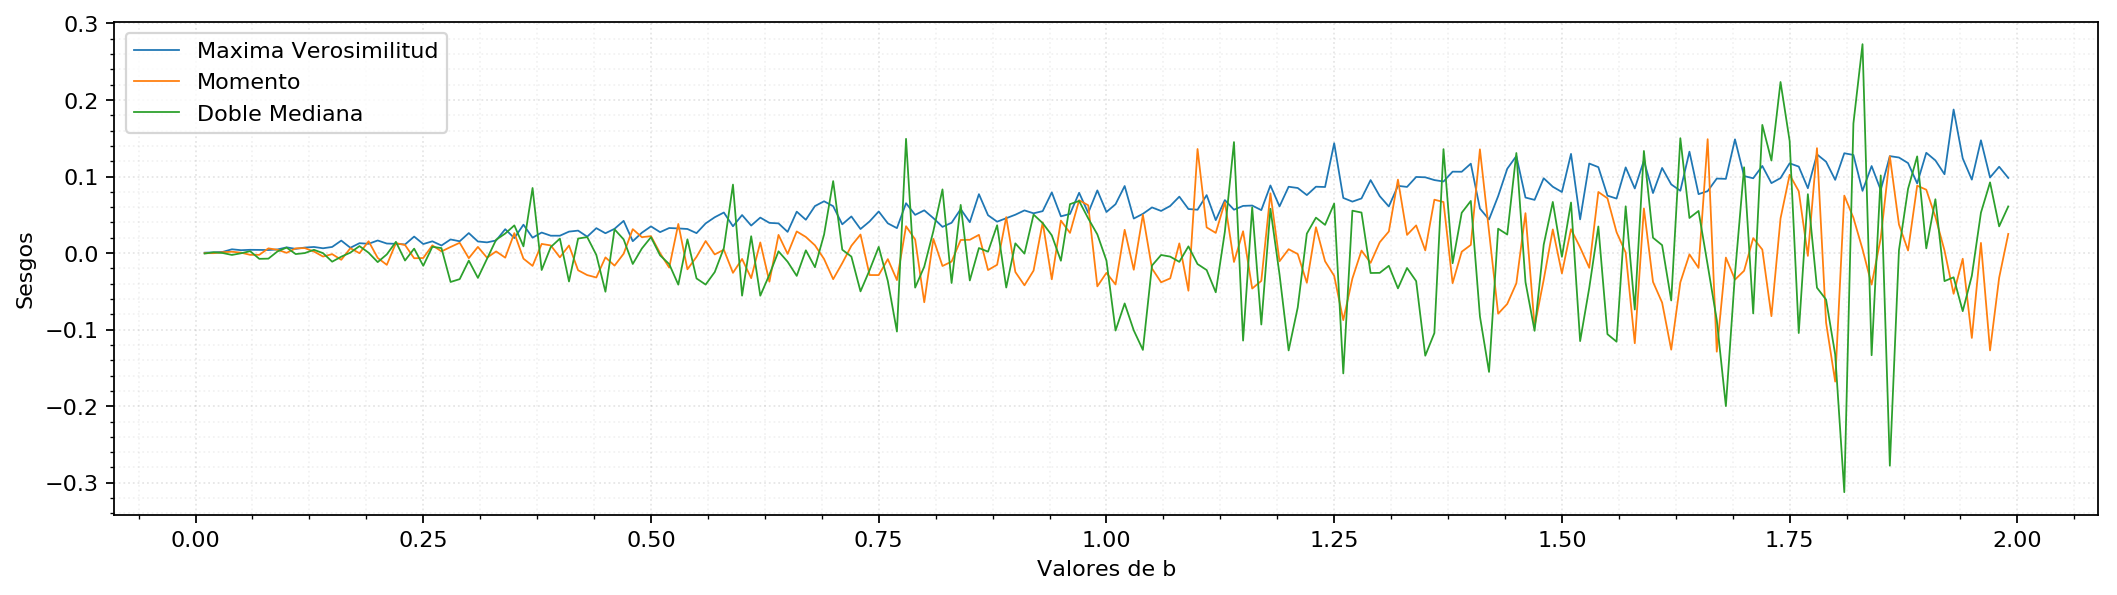
\includegraphics[width=1\textwidth]{imagenes/sesgos.png}
	\caption{\footnotesize Sesgos de los estimadores en función de los valores de \textbf{b}. $a=0, n=15$}
	\label{fig:ej6-sesgos}
\end{figure}

En la figura \ref{fig:ej6-sesgos} se puede observar que, a medida que el valor de $b$ aumenta, el valor absoluto del sesgo del estimador de $b$ también incrementa. Esto tiene sentido porque, al observar la figura \ref{fig:ej6-varianzas}, a medida que $b$ aumenta, la varianza de los estimadores también.

\begin{figure}[H]
	\centering
	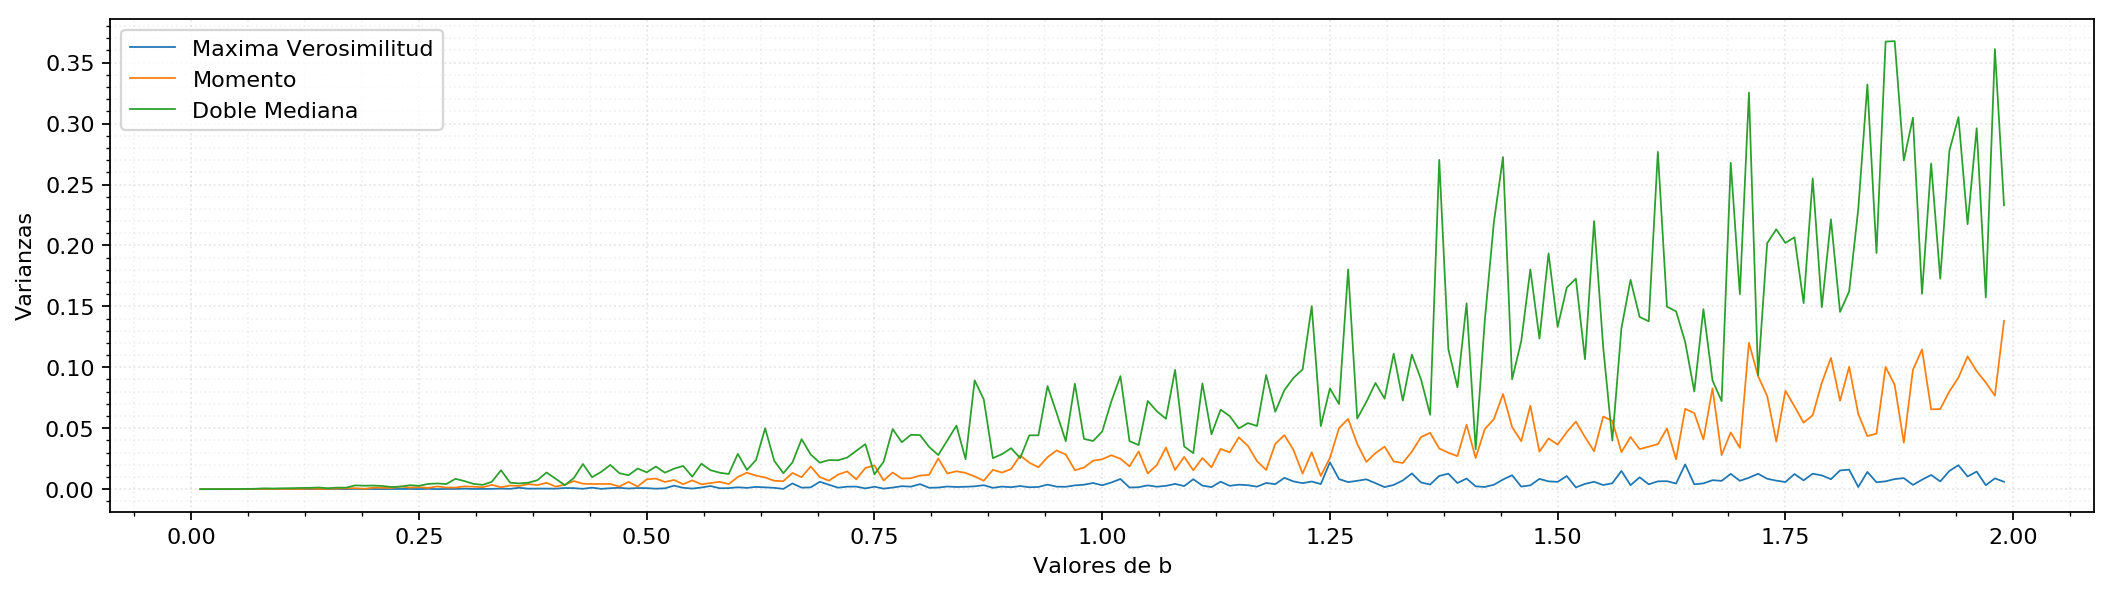
\includegraphics[width=1\textwidth]{imagenes/varianzas.png}
	\caption{\footnotesize Varianzas de los estimadores en función de los valores de \textbf{b}. $a=0, n=15$}
	\label{fig:ej6-varianzas}
\end{figure}

La figura \ref{fig:ej6-varianzas} nos muestra el comportamiento de las varianzas. Podemos observar cómo la varianza del estimador de la doble mediana $\hat{\theta}_{med}$ tiene el crecimiento máximo de entre los tres, seguida por la varianza del estimador $\hat{\theta}_{mom}$ y en último lugar, la varianza del estimador $\hat{\theta}_{mv}$. Podemos inferir que el estimador de máxima verosimilitud es el estimador de mejor calidad de entre los tres, pues su varianza no crece tan agresivamente al aumentar el valor de $b$ como en las otras alternativas.

\begin{figure}[H]
	\centering
	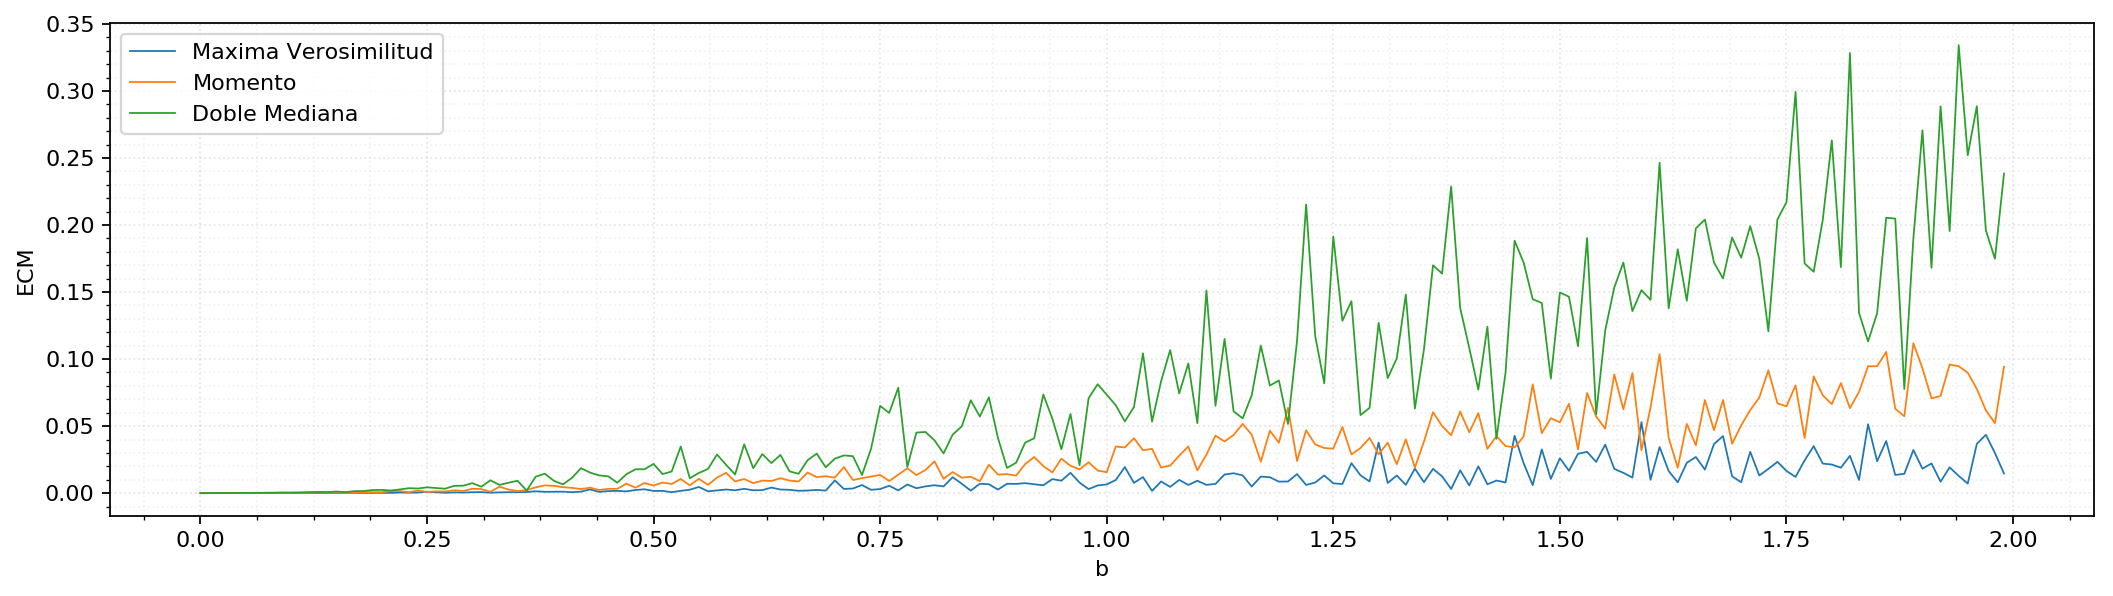
\includegraphics[width=1\textwidth]{imagenes/ecm.png}
	\caption{\footnotesize ECM de los estimadores en función de los valores de \textbf{b}. $a=0, n=15$}
	\label{fig:ej6-ecm}
\end{figure}

Finalmente, la figura \ref{fig:ej6-ecm}, complementa la conclusión llegada en los análisis anteriores. A medida que el valor de $b$ aumenta, el error cuadrático medio de cada estimador también. Podemos asegurar que el mejor estimador de los tres es el de \textbf{máxima verosimilitud}, que posee el menor crecimiento de los tres.